\documentclass[a4paper]{article}

\usepackage{amsmath,amssymb,amsfonts}
\usepackage{pgfplots}
\usepgfplotslibrary{fillbetween}
\usepackage{tikz}
\usepackage[skip=10pt plus1pt, indent=40pt]{parskip}
\pgfplotsset{width=10cm,compat=1.9}
\usepackage[makeroom]{cancel}

\def\SP#1{\textsuperscript{#1}}
\def\SB#1{\textsubscript{{#1}}}
\def\SPSB#1#2{\rlap{\textsuperscript{#1}}\SB{#2}}

\begin{document}

\begin{titlepage}
    \begin{center}
        \vspace*{1cm}

        \Huge
        \textbf{Understanding\\
          AC Power Systems\\
          Power factor}

        \vspace{0.5cm}
        \LARGE
        ...otherwise known as cos($\phi$)

        \vspace{12cm}

        \Large
        \textbf{Eric Loots}\\
        Lunatech Belgium\\
        June 27\textsuperscript{th}, 2023

    \end{center}
\end{titlepage}

In European alternating current (AC) systems, the polarity of the line
voltage cycles 50 times per second (50 Hz) following a sinusoidal curve.
This means that each cycle takes 20 ms.

When a load is connected to an AC line, the current will in general also
be sinusoidal, but it may be shifted in phase by an angle $\phi$ (We'll
get back to this later in this document as in the most general case,
current and voltage may deviate from a pure sinusoidal form).

With respect to the phase angle, three cases can be distinguished:

\begin{itemize}
	\item $\phi$ = 0 for a resistive load. Examples of this is an electrical heater system or an incandescent lightbulb.
	\item $\phi$ $>$ 0 for inductive loads. The current lags the voltage. This is the case for electrical motors or coils.
	\item  $\phi$ $<$ 0 for capacitive loads. The current precedes the voltage. This is the case for capacitors and battery chargers.
\end{itemize}\

In the most general case, a load acts as a combination of a resistive
and a reactive part, where the latter is either capacitive or inductive.

The following graph shows a line voltage and its current plotted over time. In
this case, the current lags the voltage by a 60 degrees ($\pi$/3 radians) angle,
the so-called phase angle.

\vspace{20pt}

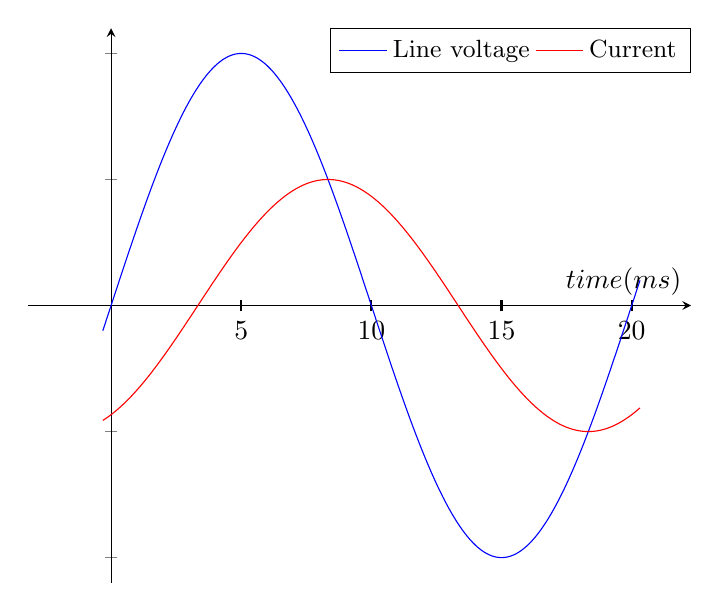
\begin{tikzpicture}
  \begin{axis}[
    ymin=-1.1, ymax=1.1,
    xmin=-1, xmax=7.0,
    axis x line=middle,
    axis y line=middle,
    xlabel=$time (ms)$,
    ylabel=$$,
    xtick={0.0, 1.5708, 3.1415, 4.7124, 6.2832},
    xticklabels={0, 5, 10, 15, 20},
    yticklabels={},
    every x tick/.style={color=black, thick},
    domain=-0.1:2*pi+0.1,
    legend style={at={(1,1)},anchor=north east,font=\small},
    legend columns=2,
  ]
    \addplot+[samples=200, mark=no] {sin(deg(x))};
    \addplot+[samples=200, mark=no] {0.5*sin(deg(x)-60)};
    \legend{
       Line voltage,
       Current,
    }
  \end{axis}
\end{tikzpicture}

At any one point in time, the instantaneous power $P_t$, is the product of
the voltage $U_t$ and current $I_t$ at that time:

\begin{align*}
   P(t) = U(t) * I(t)\
\end{align*}

We can calculate the average power over one cycle T as follows:

\begin{equation} \label{eq:realPower}
  P\SB{real} = \frac{1}{T} \int_0^{T}{P(t)} dt\\
\end{equation}\

In the case of pure sinusoidal wave forms, we have:

\begin{align*}
  U(t) &= U\SB{peak} * sin(2\pi ft)\\
  I(t) &= I\SB{peak} * sin(2\pi ft - \phi)\\
\end{align*}\

and the instantaneous power is:

\begin{equation} \label{eq:InstPower}
  P(t) = U\SB{peak} * I\SB{peak} * sin(2\pi ft) * sin(2\pi ft - \phi)\\
\end{equation}\

We can now calculate the average (real) power by putting (\ref{eq:InstPower}) into
(\ref{eq:realPower}):

\begin{equation} \label{realPower}
  P\SB{real} = U\SB{peak} * I\SB{peak} * \frac{1}{T} \int_0^{T}{sin(2\pi ft) * sin(2\pi ft - \phi)} dt\\
\end{equation}\

For simplicity, we can reason about the power by ignoring the fact that we
are working with voltages and currents. We can even abstract away the
frequency (or cycle period) and consider simple sine curves in a single
cycle of 2$\pi$ radians.

We want to calculate the average effective power of two sine waves that are out of phase by an angle of $\phi$.\

This can be expressed as:\

\begin{align*}
  P_{real} &=\frac{1}{2 \pi}\int_0^{2\pi}\sin{x} * \sin{(x - \phi)}dx\\
\end{align*}

We transform the integral using these base trigonometric identities:

\begin{align*}
  \cos{(\alpha - \beta}) &= \cos{(\alpha)} cos{(\beta)} +  \sin{(\alpha)} sin{(\beta)}\\
  \cos{(\alpha + \beta}) &= \cos{(\alpha)} cos{(\beta)} -  \sin{(\alpha)} sin{(\beta)}\\
\end{align*}

Subtracting these gives:

\begin{align*}
  \cos{(\alpha - \beta}) - \cos{(\alpha + \beta}) &= 2 \sin{(\alpha)} sin{(\beta)}\\
\end{align*}

or:

\begin{align*}
  \sin{(\alpha)} sin{(\beta)} = \frac{1}{2} (\cos{(\alpha - \beta}) - \cos{(\alpha + \beta}))
\end{align*}

Hence:

\begin{align*}
  \sin{(x)} sin{(x -\phi)} = \frac{1}{2} (\cos{(\phi}) - \cos{(2 x - \phi}))
\end{align*}

Applying this to P\SB{real}, we get:

\begin{align*}
  P\SB{real} &= \frac{1}{2 \pi}\int_0^{2\pi}\sin{(x)} * \sin{(x - \phi)}dx\\
  &= \frac{1}{4\pi}\int_0^{2\pi}\cos{(\phi}) dx - \frac{1}{4\pi}\cancelto{0}{\int_0^{2\pi}\cos{(2 x -\phi}) dx}\\
  &= \frac{1}{4\pi}\cos{(\phi})\int_0^{2\pi} dx\\
  &= \frac{1}{4\pi}\cos{(\phi}) \bigg[x \bigg]_{0}^{2\pi} dx\\
  &= \frac{1}{4 \cancel{\pi}}\cos{(\phi}) 2\cancel{\pi}\\
  &= \frac{\cos(\phi)}{2}
\end{align*}\

We get the final result in which we observe the appearance of
the infamous cos($\phi$) factor:

\begin{align*}
  P\SB{real} &=\frac{1}{2 \pi}\int_0^{2\pi}\sin{x} * \sin{(x - \phi)}dx = \frac{\cos{\phi}}{2}\\
\end{align*}\

If we bring this into the domain of the calculation of the real power,
we get:

\begin{equation}
\boxed{
\begin{aligned}
  P\SB{real} &= U\SB{peak} * I\SB{peak} * \frac{1}{T} \int_0^{T}{sin(2\pi ft) * sin(2\pi ft - \phi)} dt\\
  &= U\SB{peak} * I\SB{peak} * \frac{\cos{\phi}}{2}
\end{aligned}
}
\end{equation}

Some readers may have heard about (AC) RMS voltages and currents. If
you've ever measured, or saw anyone measuring voltages or currents using a
multimeter or current probes, the devices would carry a label "True RMS
Meter". So, what does RMS stand for and what is its definition?

RMS is the acronym for "Root Mean Square", and for a periodic wave V(t) with
period T, it's defined as follows:

\begin{align*}
  V\SB{RMS} &= \sqrt{\frac{1}{T} \int_0^{T} V\SP{2}(t) dt}\\
\end{align*}\

Applying this for a pure sinusoidal waveform, this gives:

\begin{align*}
  V\SB{RMS} &= \sqrt{\frac{1}{2 \pi} \int_0^{2 \pi} (V\SB{peak} * sin(\phi))\SP{2} d\phi}\\
  &= \sqrt{\frac{V\SPSB{2}{peak}}{2 \pi} \int_0^{2 \pi} sin\SP{2}(\phi) d\phi}\\
  &= V\SB{peak} * \sqrt{\frac{1}{2 \pi} \int_0^{2 \pi} sin\SP{2}(\phi) d\phi}\\
\end{align*}

We already encountered the integral of $\sin\SP{2}(\phi)$ in this article.
It evaluates to $\pi$ so that we obtain:

\begin{align*}
  V\SB{RMS} &= V\SB{peak} * \sqrt{\frac{\pi}{2 \pi}}\\
  &= \frac{V\SB{peak}}{\sqrt{2}}\\
\end{align*}

Similarly, we get a formula for $I\SB{RMS}$:

\begin{align*}
  I\SB{RMS} &= \frac{I\SB{peak}}{\sqrt{2}}\\
\end{align*}

Substituting the RMS values for the peak values in the formula for
$P\SB{real}$, we get the final, very simple and important result:

\begin{equation*}
  \begin{aligned}
  P\SB{real} &= V\SB{peak} * I\SB{peak} * \frac{\cos{\phi}}{2}\\
  &= \frac{V\SB{peak}}{\sqrt{2}} * \frac{I\SB{peak}}{\sqrt{2}} * \cos{\phi}\\
  \end{aligned}
\end{equation*}

or:

\begin{equation} \label{eq:cosPhi}
   \boxed{
	P\SB{real} = V\SB{RMS} * I\SB{RMS} * \cos{\phi} \\
   }
\end{equation}

With $V\SB{RMS} * I\SB{RMS}$ being $P\SB{apparent}$, we  see that:

\begin{align*}
  P\SB{real} &= P\SB{apparent} * \cos{\phi} \\
\end{align*}

If we define $P\SB{reactive}$ to be:

\begin{align*}
  P\SB{reactive} &= P\SB{apparent} * \sin{\phi} \\
\end{align*}

We also see that:

\begin{align*}
  P\SPSB{2}{apparent} &= P\SPSB{2}{real} + P\SPSB{2}{reactive} \\
\end{align*}

Even though $\cos(\phi)$ in (\ref{eq:cosPhi}) has been derived for pure
sinusoidal waveforms, the concept can be generalised for arbitrary
periodic waveforms. One can always calculate the RMS values for the
voltage and current from which the apparent power can be calculated.
The real power can be calculated using (\ref{eq:realPower}). With $P\SB{real}$
and $P\SB{apparent}$, we can define $\cos(\phi)$ as follows:

\begin{align*}
  \cos(\phi) = \frac{P\SB{real}}{P\SB{apparent}}
\end{align*}

To get a more intuitive feel for what apparent and real power are, I added
figures 1 and 2, in which we plot the voltage and current waveforms for the cases
where $\phi = 0$ \emph{a purely "resistive load"}, and $\phi = \pi / 2$ \emph{a 
purely "inductive load"} .
The instantaneous power in the former case is always positive,
whereas in the inductive case it's alternately positive and negative.
The physical interpretation is that for a resistive load, the direction of
energy transfer is from the generation side to the consumption side. For
the purely inductive load case, energy flows in equal amounts from and
to the producer and the load. The effect is that, on balance, no net energy
is transferred between the two and there's just energy "bouncing" between
opposite ends.

\begin{figure}
  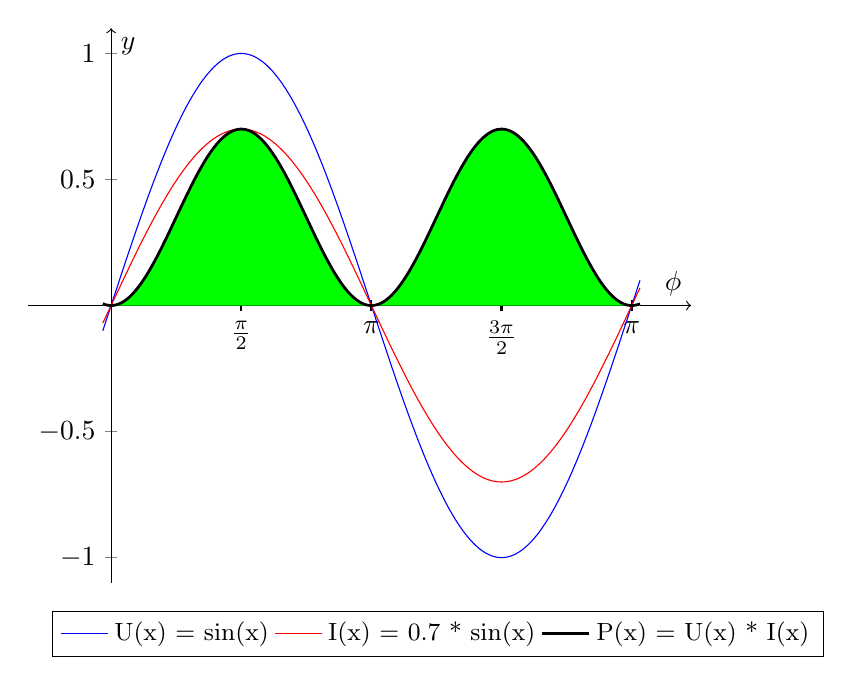
\begin{tikzpicture}
    \begin{axis}[
      ymin=-1.1, ymax=1.1,
      xmin=-1, xmax=7,
      axis x line=middle,
      axis y line=middle,
      axis line style={->},
      %xtick distance = pi,
      xlabel=$\phi$,
      ylabel=$y$,
      %ylabel={$f(x) = sin(x)^2 - x +9$},
      xtick={0, 1.5708, 3.1415, 4.7124, 6.2832},
      xticklabels={0, $\frac{\pi}{2}$, $\pi$, $\frac{3\pi}{2}$, $\pi$},
      domain=-0.1:2*pi+0.1,
      every x tick/.style={color=black, thick},
      legend style={at={(1.2,-0.05)},anchor=north east,font=\small},
      legend columns=3,
    ]
      \addplot+[samples=200, mark=no] {sin(deg(x)};
      \addplot+[samples=200, mark=no] {0.7 * sin(deg(x)};
      \addplot+[line width=1pt, color=black, samples=200, mark=no, name path = A] {sin(deg(x)) * 0.7 * sin(deg(x))};
      \addplot+[draw=none,name path=B, mark=no] {0};
      \addplot+[green] fill between[of=A and B];
      \legend{
              U(x) = sin(x),
              I(x) = 0.7 * sin(x),
              P(x) = U(x) * I(x)
      }
    \end{axis}
  \end{tikzpicture}
  \caption{Perfect resistive load case}\label{fig:powerResistive}
  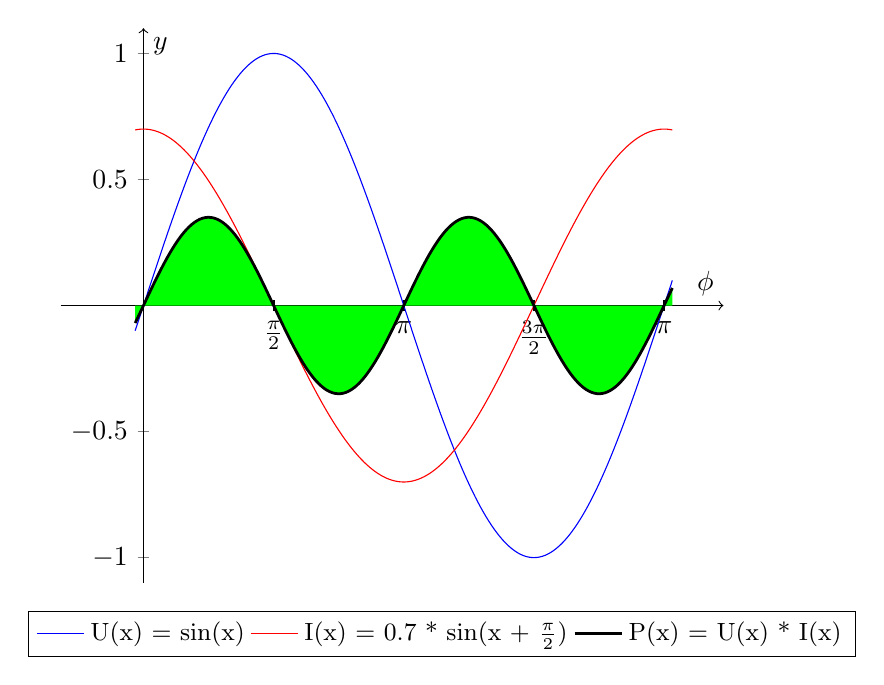
\begin{tikzpicture}
    \begin{axis}[
      ymin=-1.1, ymax=1.1,
      xmin=-1, xmax=7,
      axis x line=middle,
      axis y line=middle,
      axis line style={->},
      %xtick distance = pi,
      xlabel=$\phi$,
      ylabel=$y$,
      %ylabel={$f(x) = sin(x)^2 - x +9$},
      xtick={0, 1.5708, 3.1415, 4.7124, 6.2832},
      xticklabels={0, $\frac{\pi}{2}$, $\pi$, $\frac{3\pi}{2}$, $\pi$},
      domain=-0.1:2*pi+0.1,
      every x tick/.style={color=black, thick},
      legend style={at={(1.2,-0.05)},anchor=north east,font=\small},
      legend columns=3,
    ]
      \addplot+[samples=200, mark=no] {sin(deg(x)};
      \addplot+[samples=200, mark=no] {0.7 * sin(deg(x)+90};
      \addplot+[line width=1pt, color=black, samples=200, mark=no, name path = A] {sin(deg(x)) * 0.7 * sin(deg(x)+90)};
      \addplot+[draw=none,name path=B, mark=no] {0};
      \addplot+[green] fill between[of=A and B];
      \legend{
              U(x) = sin(x),
              I(x) = 0.7 * sin(x + $\frac{\pi}{2}$),
              P(x) = U(x) * I(x)
      }
    \end{axis}
  \end{tikzpicture}
  \caption{Perfect capacitive load case}\label{fig:powerInductive}
\end{figure}

\end{document}